\graphicspath{{figures/design/}}
\chapter{Design}\label{ch:design}
This chapter gives an in-depth description of how implementations are made. \todo{More intro}

\section{Preprocessing}
To be able to do object detection, image preprocessing is necessary. Because fo the high contrast between the background and the fish due to the \gls{nir} background lighting, background subtraction is not necessary. 

The preprocessing is done in three steps:

\begin{itemize}
	\item Greyscale conversion
	\item Noise reduction
	\item Thresholding
\end{itemize}

\subsubsection{Greyscale conversion}
Using OpenCV each image is converted to greyscale using the reference image.

\begin{figure}[H]
	\centering
	\begin{subfigure}[b]{0.43\textwidth}
		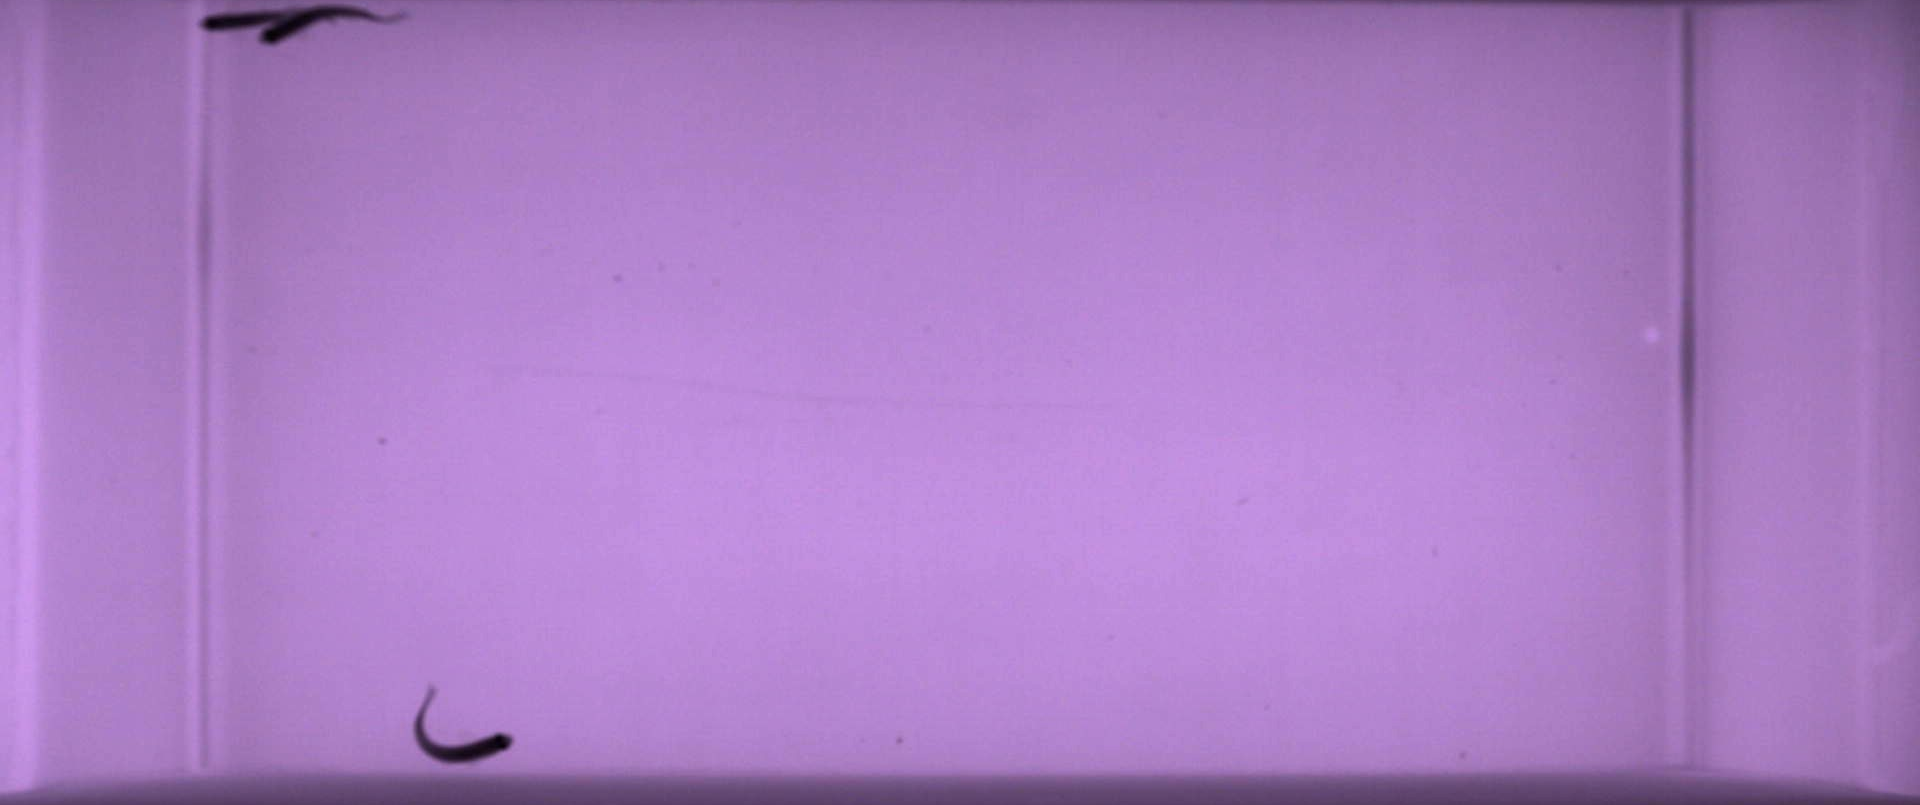
\includegraphics[width=\textwidth]{image.png}
		\caption{Original image of three fish}
		\label{fig:grey_orig}
	\end{subfigure}
	\begin{subfigure}[b]{0.43\textwidth}
		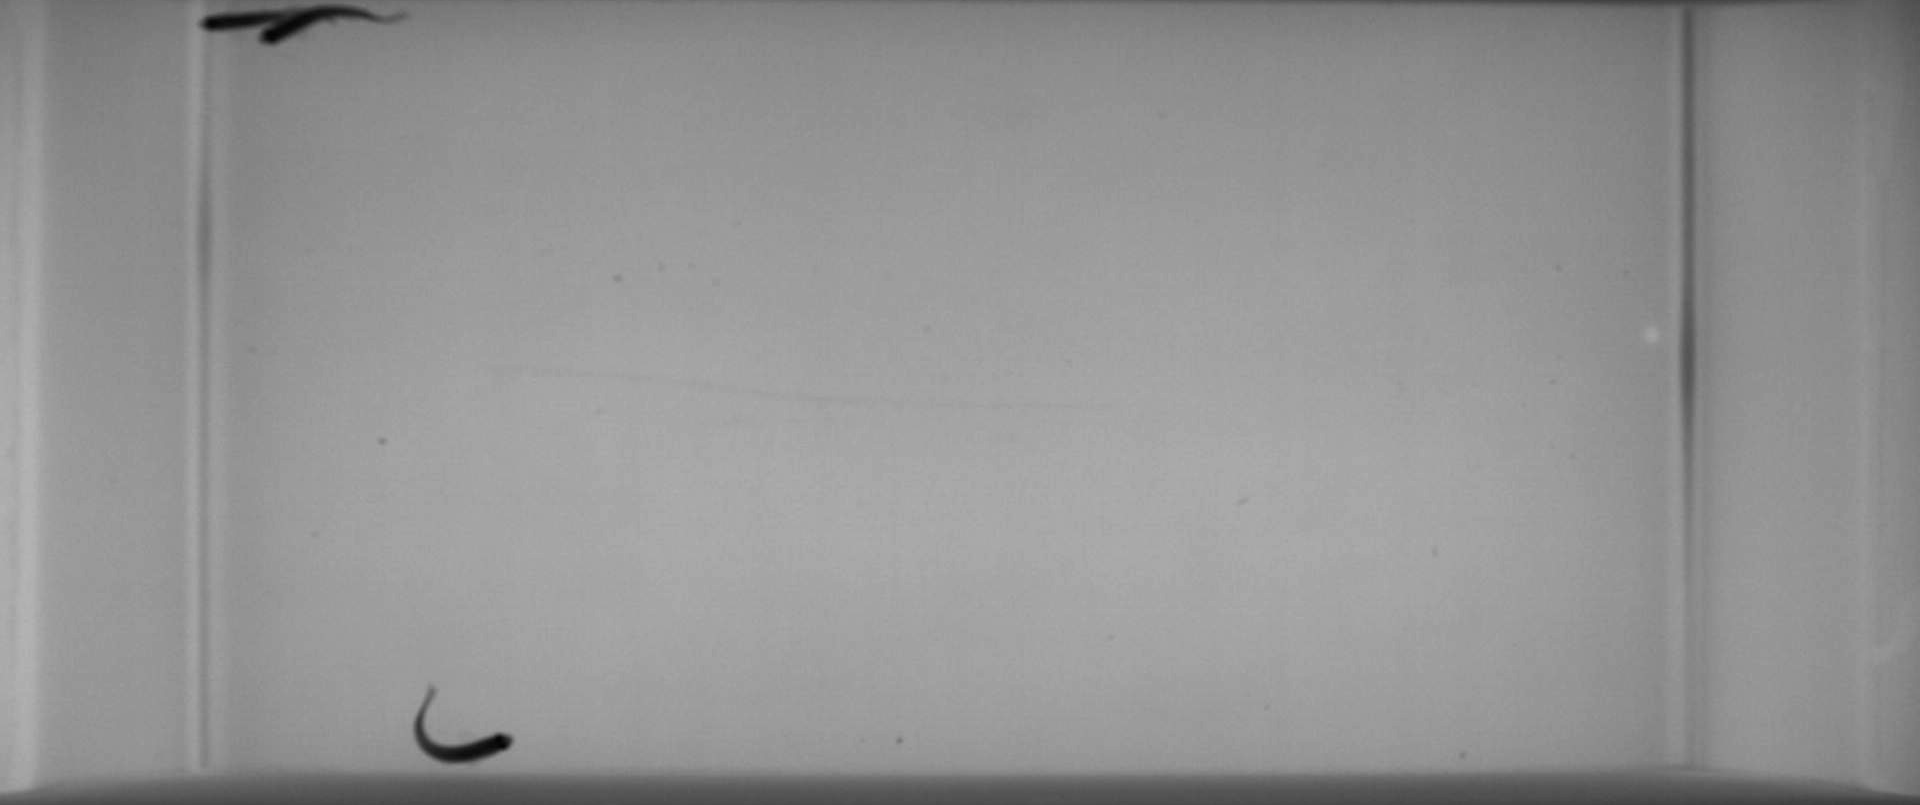
\includegraphics[width=\textwidth]{grey.png}
		\caption{Grey scale image of three fish}
		\label{fig:grey}
	\end{subfigure}
	\label{fig:orig_to_grey}
\end{figure}

\subsubsection{Noise reduction}
To enhance edges of the fish some noise reduction is done using a Gaussian smoothing kernel, included in OpenCV. The kernel size is set to $5 \times 5$, and the standard Gaussian deviation is calculated from the kernel size (ksize):

\begin{equation}
	\sigma = 0.3\*((ksize-1)\*0.5 - 1) + 0.8
\end{equation}

\begin{figure}[H]
	\centering
	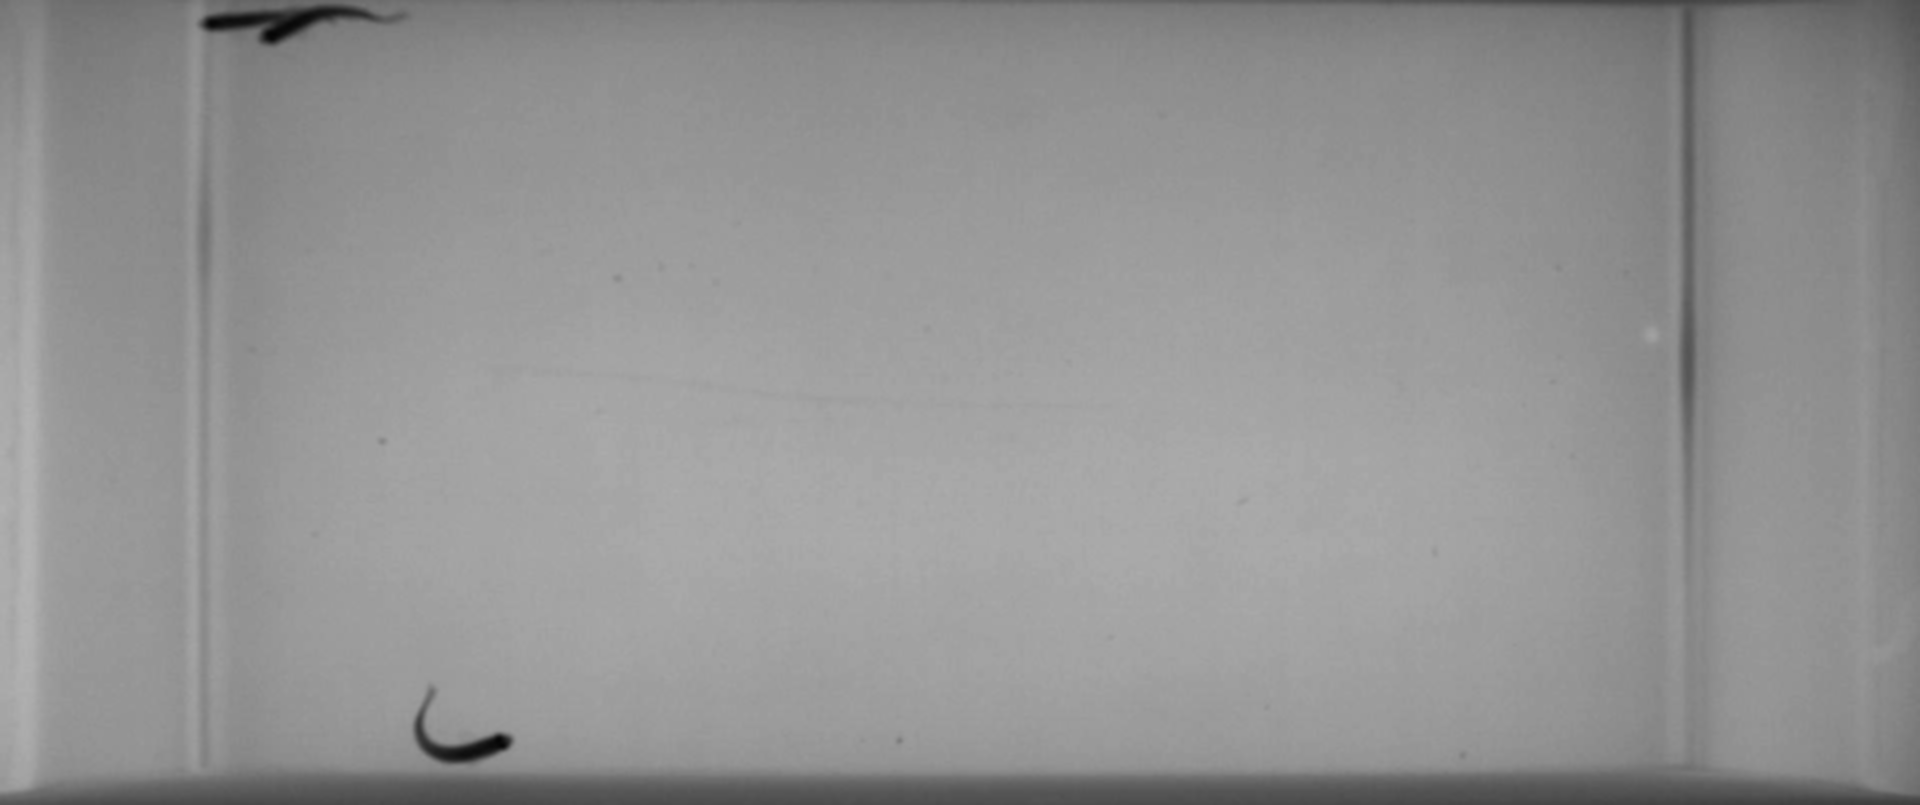
\includegraphics[width=0.5\textwidth]{blurred.png}
	\caption{Gray imaged after Gaussian smoothing}
	\label{fig:blurred}
\end{figure}

There is not much difference to be seen by the naked eye, but the image background is a bit brighter and the pixel values have changed.

\subsubsection{Thresholding}
Thresholding is used to remove all unwanted pixels from the image to be able to recognise BLOBs. Because of the high contrast between the background and the fish, with the fish being very dark opposed to everything else in the image, a threshold is set close to the darkest pixels in the image.
The threshold is set at a pixel of $35$ which eliminates everything else than the fish BLOBs as shown in \autoref{fig:thresh}. After the threshold, the values are inverted.

\begin{figure}[H]
	\centering
	\begin{subfigure}[b]{0.3\textwidth}
		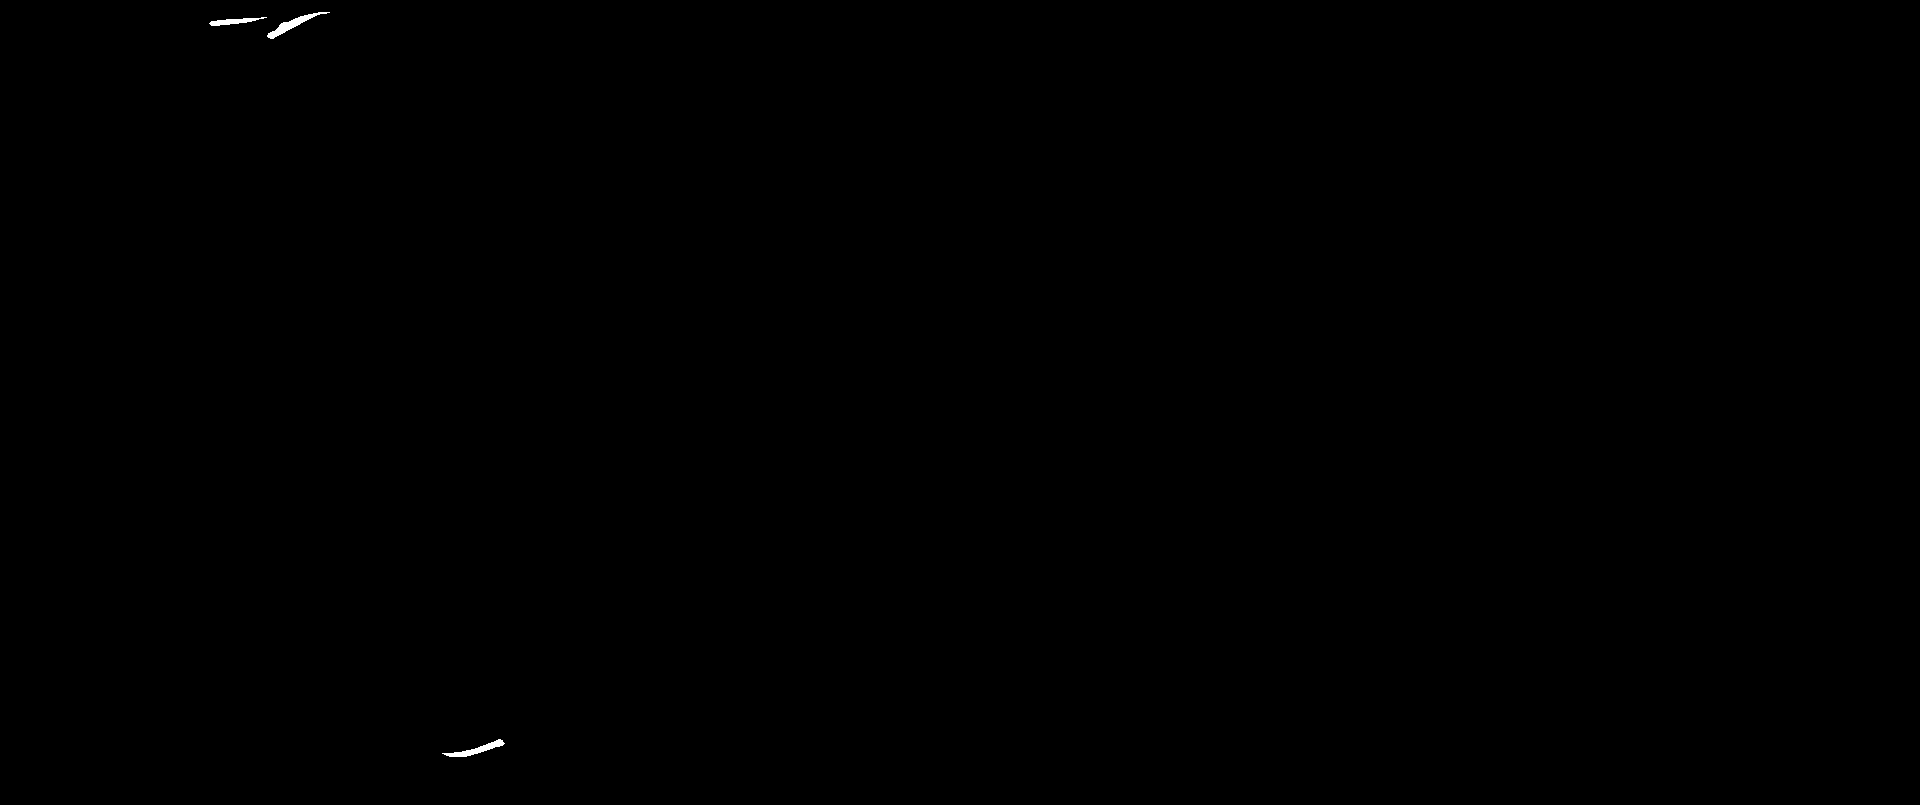
\includegraphics[width=\textwidth]{thresh35.png}
		\caption{Threshold at a pixel value of 35}
		\label{fig:thresh35}
	\end{subfigure}
	\begin{subfigure}[b]{0.3\textwidth}
		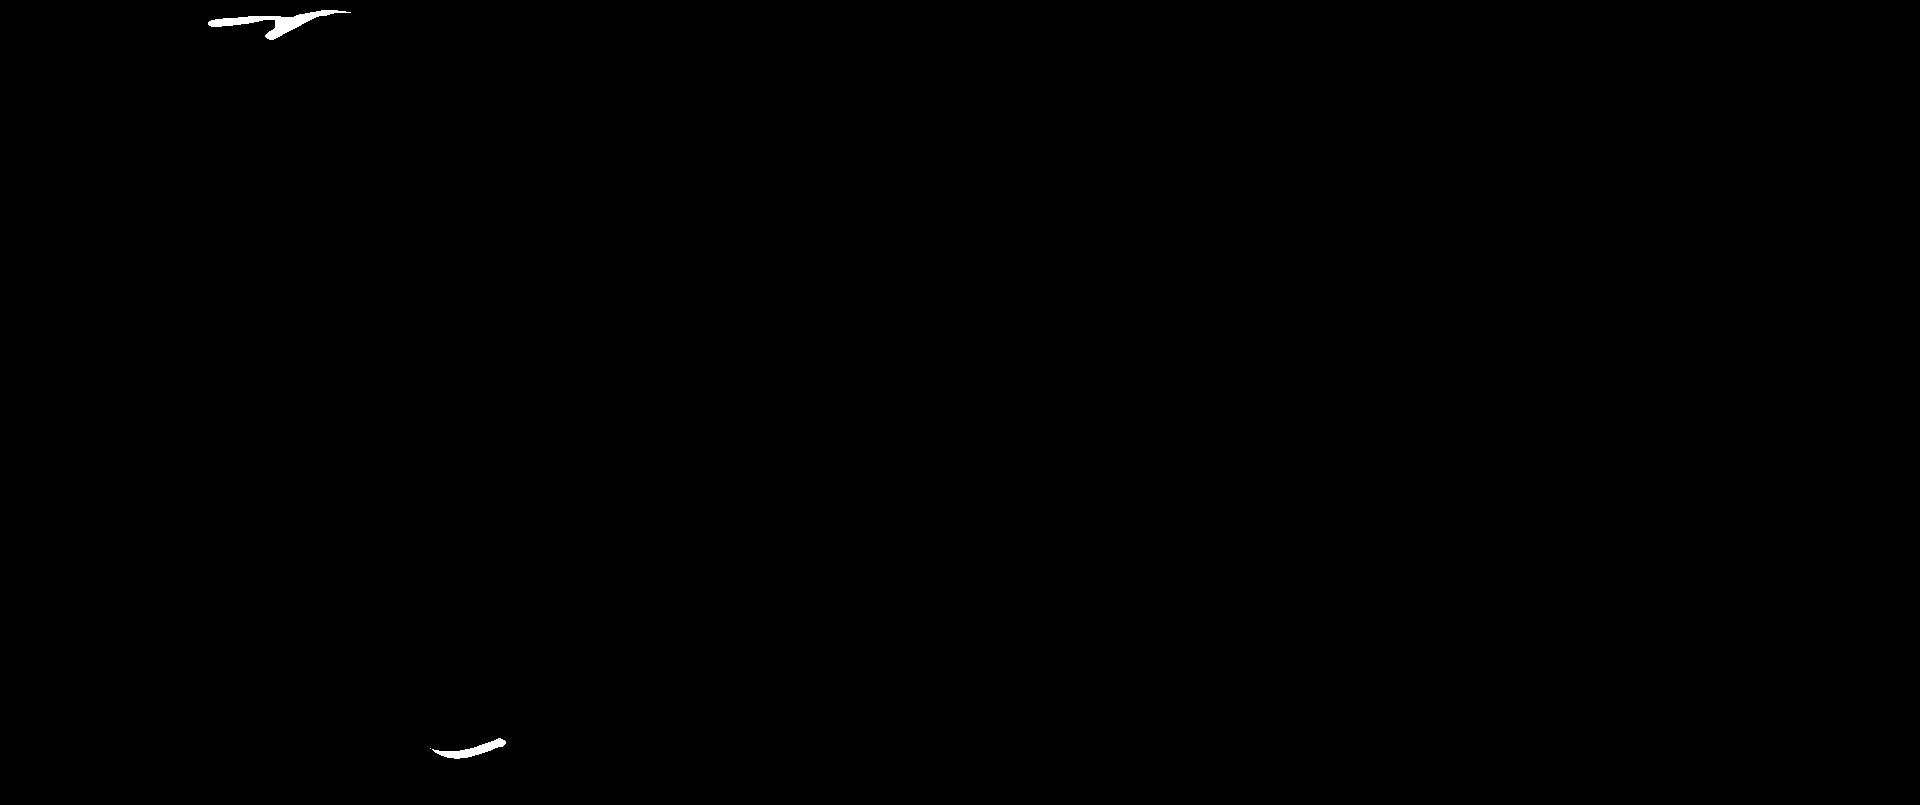
\includegraphics[width=\textwidth]{thresh50.png}
		\caption{Threshold at a pixel value of 50}
		\label{fig:thresh50}
	\end{subfigure}
	\begin{subfigure}[b]{0.3\textwidth}
		
\includegraphics[width=\textwidth]{thresh70.png}
		\caption{Threshold at a pixel value of 70}
		\label{fig:thresh70}
	\end{subfigure}
	\caption{Different threshold levels}
	\label{fig:thresh}
\end{figure}

The three images show different levels of thresholds. Even though only the fish are visible at a pixel value of $50$, the two fish are creating just one BLOB, whereas at $35$ some erosion of is done, and the two fish are separated.

With the BLOBs clear in the image, object detection is the next step.

\section{Object Detection}
With the binary image, BLOB extraction is straight forward. As the image is without any noise due to the high contrast, detections are searching for ones in a space of zeroes.

To detect an object, each BLOB needs to be identified individually. By contouring each BLOB, each fish is outlined, but the contouring function from OpenCV also identifies each BLOB as an individual.

Another approach to detecting each BLOB is by skeletonising each BLOB. With the fish, this will end up in a single spine marking line.

\subsection{Find Contour}
The contouring algorithm follows the approach presented in \cite{Suzuki1985}. The algorithm iterates through a binary image, checking for borders, both outer borders of BLOBs and hole borders. As there are only solid BLOBs in the images, hole borders are not detected by the algorithm as it requires a complete circling of 1-pixels around a hole of 0-pixels.

By tagging pixels, the algorithm keeps track on which category or BLOB the pixels belongs to. One pixel can change from being recognised as an outer border to a hole border if a both categories are applicable to the one pixel. The iteration process is making use of 4-connectivity to detecting continuous border after finding the first 1-pixel, whereas when iteration for a hole or background, 8-connectivity is used. An example of the connectivity is shown in \autopageref{fig:connectiv}.

\begin{figure}[H]
	\centering
	\begin{subfigure}[b]{0.4\textwidth}
		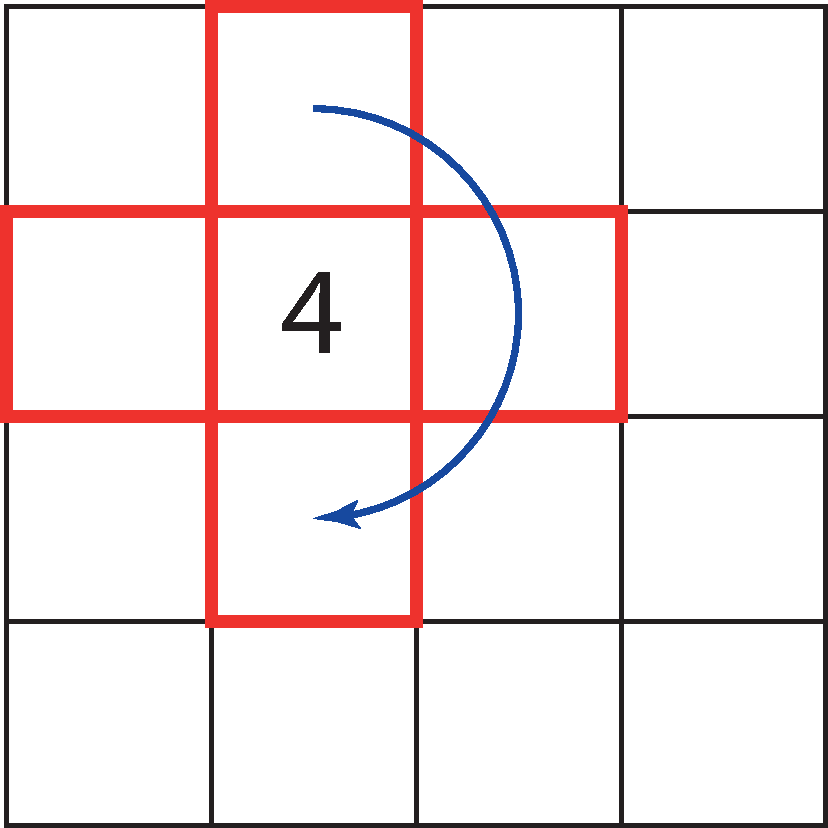
\includegraphics[width=\textwidth]{4-con.pdf}
		\caption{4-Connectivity}
		\label{fig:4-con}
	\end{subfigure}
	\begin{subfigure}[b]{0.4\textwidth}
		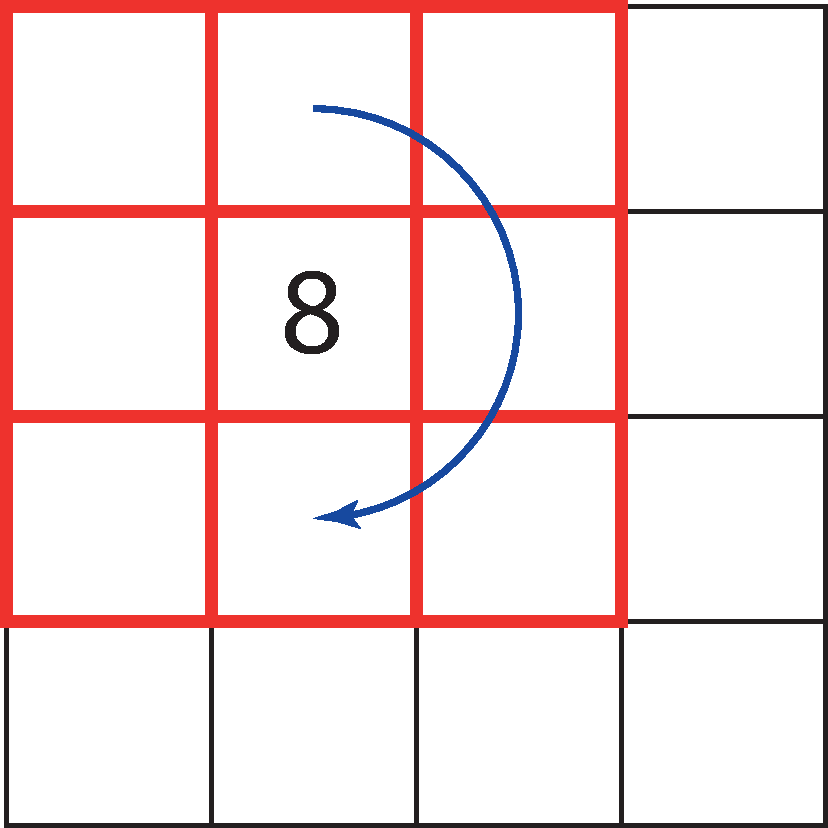
\includegraphics[width=\textwidth]{8-con.pdf}
		\caption{8-Connectivity}
		\label{fig:8-con}
	\end{subfigure}
	\caption{4- and 8-connectivity as used in the algorithm}
	\label{fig:connectiv}
\end{figure}

When a contour of a BLOB is fully connected, it is tagged as a surface $ S $. The contour marked is the outermost 1-pixels of each BLOB.

\subsection{Skeletonisation}
To gather some characteristics of each BLOB, a skeletonisation is done on each image. With this information, it is possible to find both simpler coordinates of each BLOB instead of a contour, but the skeleton can also show characteristics of a BLOB consisting of two fish or more if they are not straight on top of each other.

The function is included in the \textit{skimage} package for Python and is based on article by \cite{Zhang1984}. The function is a thinning algorithm, which thins a BLOB until a pre set thickness of each BLOB is reached. This means the contour points are removed from the image in each iteration. In ehac itertaion, the contour point is denoted $P_1$. 
To preserve connectivity of the skeleton, each iteration is split into two subiterations. The firs subiteration has four conditions to fulfil:

\begin{itemize}
	\item[a)] $ 2 \leq B(P_1) \leq 6 $
	\item[b)] $ A(P_1) = 1 $
	\item[c)] $ P_2 \cdot P_4 \cdot P_6 = 0 $
	\item[d)] $ P_4 \cdot P_6 \cdot P_8 = 0 $
\end{itemize}

Here $B(P_1)$ is the amount of non-zero neighbours of $P_1$ in 8-connectivity. $ A(P_1) $ is the amount of $01$ patterns in the ordered set $P_2, P_3, ... , P_9$, which are the eight neighbours of $P_1$. An example of a pattern not fulfilling this condition is shown in \autoref{fig:01pattern} as the condition of having only one occurrence of the pattern is not fulfilled with $A(P_1) = 2$.

The result of this is that $P_1$ is not removed.

\begin{figure}[H]
	\centering
	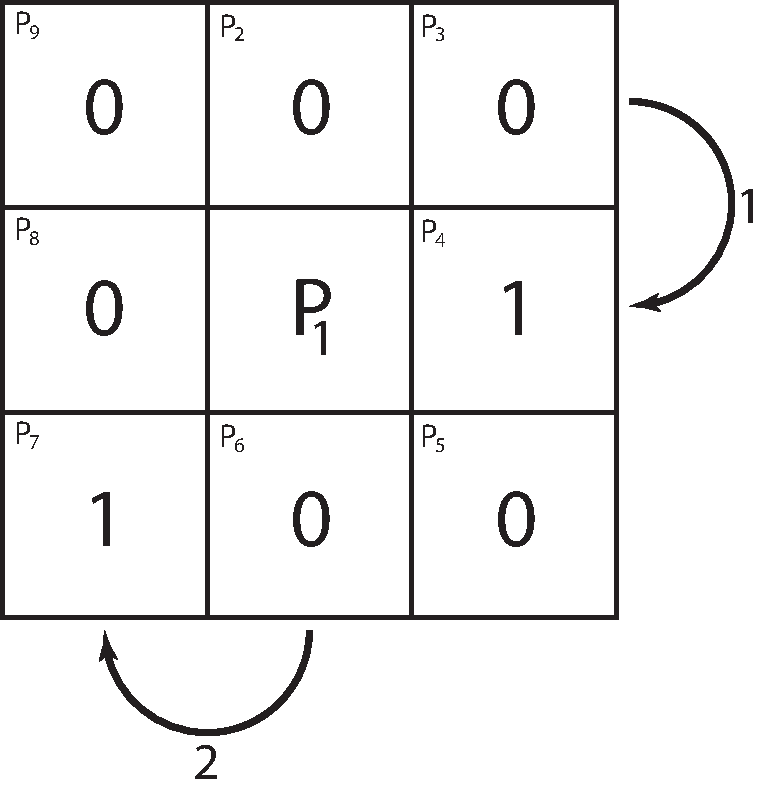
\includegraphics[width=0.5\textwidth]{01pattern}
	\caption{A $01$ pattern not fulfilling condition b) of the thinning algorithm used for skeletonisation. Inspired from \cite{Zhang1984}}
	\label{fig:01pattern}
\end{figure}

The second subiteration has a change to the two last conditions, but the two first conditions remain the same;

\begin{itemize}
	\item[c')] $ P_2 \cdot P_4 \cdot P_8 = 0 $
	\item[d')] $ P_2 \cdot P_6 \cdot P_8 = 0 $
\end{itemize}

The first subiteration is only capable of removing north-west corner points and the south-east boundary points. Whereas the second subiteration is only capable of removing a north-west boundary point and a south-east corner point. The condition a) is responsible of keeping skeleton line endpoints, and condition b) prevents removal of points between endpoints of the skeleton lines \citep{Zhang1984}. The two instances are shown in \autoref{fig:endpoint}.

\begin{figure}[H]
	\centering
	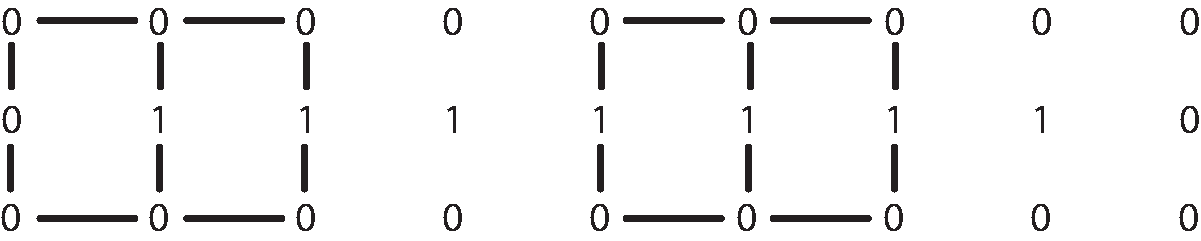
\includegraphics[width=0.85\textwidth]{endpoint}
	\caption{Endpoint preservation example made possible from conditions a) and b). Example remade from \cite{Zhang1984}}
	\label{fig:endpoint}
\end{figure}

\autoref{fig:endpoint} shows that neither condition a) or b) are fulfilled, which results in preservation of the endpoint and avoids loss of a connection to the endpoint.\\

With the known positions of the BLOBs and the skeletons extracted, interaction between the fish causing occlusions can be found.
\section{Occlusion Detection}
With the known positions of the BLOBs and the each fo their skeletons extracted, occlusions can be found in at least two different ways.

Using contours of the BLOBs the amount of BLOBs or contours can be counted and by knowing the amount of fish in the water, occlusions can, in general, be found by counting BLOBs.

Another solution is by using the skeletons by searching for intersections in the skeletons, to see if a skeleton is splitting out into two branches, which would indicate a crossing of bodies.\\

An occlusion is defined as two fish or more covering one another which will decrease the amount of BLOBs in the image. An example of this in both colour and binary is shown in \autoref{fig:occlusion_example}.

\begin{figure}[H]
	\centering
	\begin{subfigure}{0.45\textwidth}
		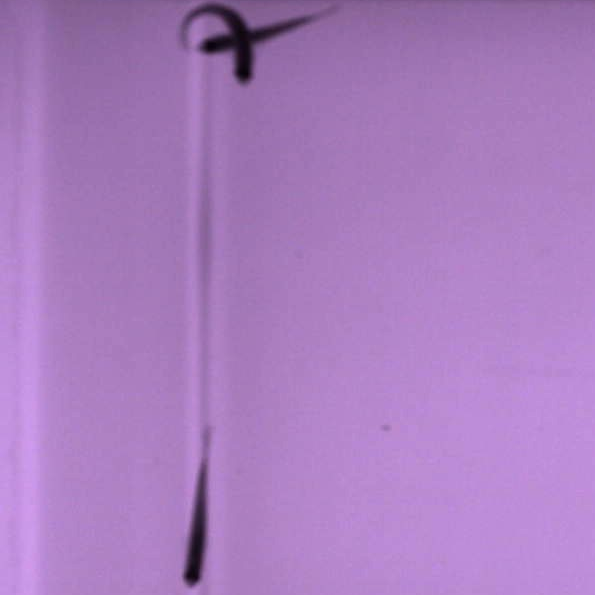
\includegraphics[width=\textwidth]{occl_colour}
		\caption{Colour example of an occlusion. The example is cut to the area including the fish}
		\label{fig:occl_colour}
	\end{subfigure}
	\begin{subfigure}{0.45\textwidth}
		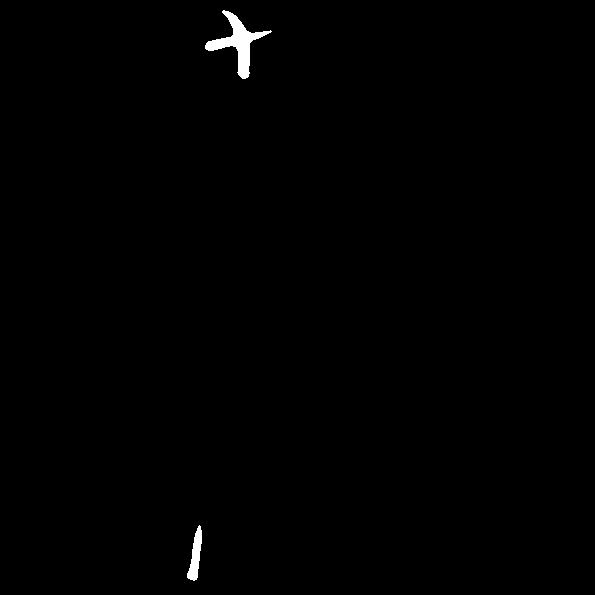
\includegraphics[width=\textwidth]{occl_binary}
		\caption{Binary example of an occlusion. The example is cut to the area including the fish}
		\label{fig:occl_binary}
	\end{subfigure}
\caption{Examples of an occlusion of one fish done by another on top}
\label{fig:occlusion_example}
\end{figure}

\subsection{Contour Counting}
As the BLOB contour implementation counts the amount of contours present in each frame of the video, it is possible to detect if there are enough BLOBs in the image to correspond to the amount of fish in the aquarium.